\documentclass[../memoria.tex]{subfiles} 
\begin{document}
\label{modelo desarrollado} 
%\renewcommand{\p@subfigure}{}% Void parent macro for figures

Este capítulo describe un prototipo de sistema de Re-ID de personas, enfocado en el procesamiento de videos de vigilancia reales en ambientes no controlados. La arquitectura en la que se basa el prototipo se puede ver en la figura \ref{fig:sistemaReID}

\section{Detección de Personas}

El sistema de Re-ID se desarrolló para trabajar con videos capturados desde cámaras inmóviles, lo que permite distinguir entre las partes de la imagen que corresponden al escenario de fondo (puntos fijos) y primer plano (puntos móviles). De ahí que el sistema se enfoca únicamente en las regiones pertenecientes al primer plano o regiones de interés, por lo que sólo se requiere seleccionar aquellas regiones de interés pertenecientes a personas. %En la sección \ref{seleccion roi} se propone un método de selección de bajo costo computacional y que saca provecho del conocimiento de que se tenga del ambiente.

\subsection{Segmentación de planos}
\label{segmentacion planos}

\begin{figure}
    \centering
      \begin{subfigure}{0.3\textwidth}
        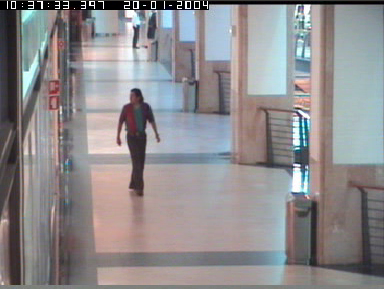
\includegraphics[width=\textwidth]{persona5a.png}
          \caption{}
          \label{fig:segmentacion:original}
      \end{subfigure}
      \hfill
      \begin{subfigure}{0.3\textwidth}
        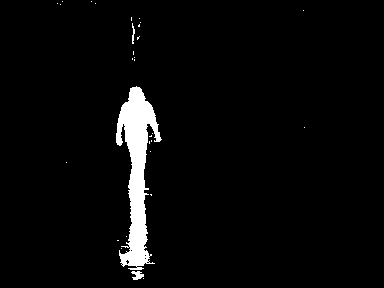
\includegraphics[width=\textwidth]{persona4b.png}
          \caption{}
          \label{fig:segmentacion:sin detec sombra}
      \end{subfigure}
      \hfill
      \begin{subfigure}{0.3\textwidth}
        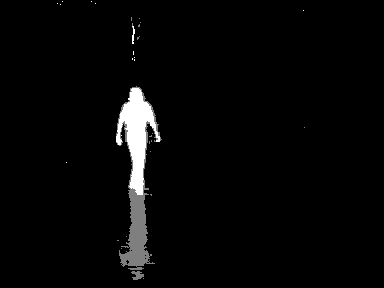
\includegraphics[width=\textwidth]{persona4c.png}
          \caption{}
          \label{fig:segmentacion:con detec sombra}
      \end{subfigure}
      \\
      \begin{subfigure}{0.3\textwidth}
        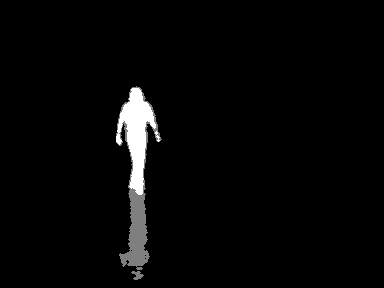
\includegraphics[width=\textwidth]{persona4d.png}
          \caption{}
          \label{fig:segmentacion:ruido filtrado}
      \end{subfigure}
      \hfill
      \begin{subfigure}{0.3\textwidth}
        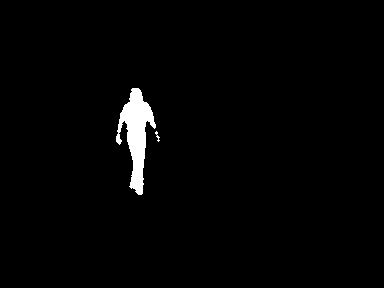
\includegraphics[width=\textwidth]{persona4e.png}
          \caption{}
          \label{fig:segmentacion:sombra filtrada}
      \end{subfigure}
      \hfill
      \begin{subfigure}{0.3\textwidth}
        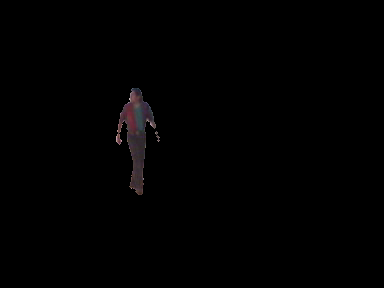
\includegraphics[width=\textwidth]{persona4f.png}
          \caption{}
          \label{fig:segmentacion:original enmascarado}
      \end{subfigure}
\caption{
\label{fig:segmentacion}
Segmentación:(a) Frame original. (b) Sin detección de sombra. (c) Con detección de sombras. (d) Ruido filtrado. (e) Sombra filtrada. (f) Frame enmascarado}
\end{figure}

Se utilizó el algoritmo de segmentación entre primer y segundo plano presentado en \cite{zivkovic2004improved,zivkovic2006efficient} que identifica los píxeles correspondientes a zonas en movimiento según los cambios producidos entre cada cuadro consecutivo del video, utilizando la distribución de probabilidad de Gauss. Esta detección genera un nuevo mapa de bits de dimensión idéntica al cuadro original y cuyos píxeles pueden ser blanco o negro para zonas en movimiento y estáticas, respectivamente (ver figura \ref{fig:segmentacion:sin detec sombra}). Sin embargo, esta primera detección es sensible a pequeños movimientos producto de vibraciones, corrientes de aire, cambios de iluminación, etc, lo que altera píxeles aislados que forman regiones conexas que no alcanzan a ser de tamaño considerable. Por esto, se utilizó un método basado en morfología mátematica\footnote{específicamente aplicando el operador de erosión, seguido por la dilatación de la imagen.} para eliminar el ruido de píxeles blancos presente en una imagen (figura \ref{fig:segmentacion:ruido filtrado}).

%Nota: no entiendo la lógica de esto
Las sombras pueden formar parte del primer plano si estás no son detectadas, lo que implica que la región de interés abarque espacio que no corresponde al cuerpo de la persona. Sin embargo, las sombras pueden ser detectadas por el mismo algoritmo de segmentación citado anteriormente. Este algoritmo puede generar un mapa de bits, esta vez con píxeles en escala de grises (ver figura \ref{fig:segmentacion:con detec sombra}), donde las sombras son representadas con valores grises. Dado que el segundo plano es representado únicamente por píxeles de color negro, eliminar la sombra del primer plano equivale a transformar el gris a negro. Esta transformación consiste en convertir todo píxel que tenga un valor menor a un umbral en cero (equivalente al negro), y todo valor mayor o igual a dicho umbral en uno (equivalente al blanco). El resultado de la aplicación de dicho umbral se puede apreciar en la figura \ref{fig:segmentacion:sombra filtrada}. Luego, se utilizó este mapa de bits como una \emph{máscara} que se sobrepone al frame, ocultando todo el segundo plano (\emph{background subtraction}). Los píxeles de cada frame (máscara y original) son operados como valores lógicos con el operador AND, considerando sus valores como secuencia de bits (ver figura \ref{fig:segmentacion:original enmascarado}).

Una vez eliminado el segundo plano, se identifican todas las formas persistentes en la imagen (regiones de interés). Para esto se considera la existencia de máximo una forma perteneciente a persona dentro de un frame. 

\subsection{Selección de la región de interés}
\label{seleccion roi}

\begin{figure}
    \centering
      \begin{subfigure}{0.45\textwidth}
        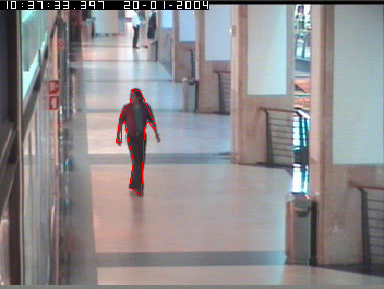
\includegraphics[width=\textwidth]{persona5b.png}
          \caption{}
          \label{fig:seleccion roi:poligono}
      \end{subfigure}
      \hfill
      \begin{subfigure}{0.45\textwidth}
        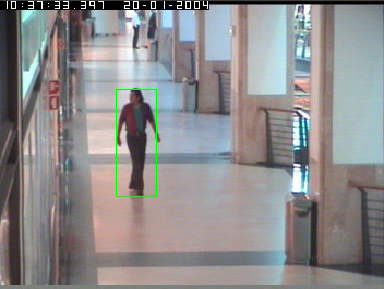
\includegraphics[width=\textwidth]{persona5c.png}
          \caption{}
          \label{fig:seleccion roi:rectangulo}
      \end{subfigure}
\caption{
\label{fig:seleccion roi}%
Región de interés:(a) Polígono que aproxima los bordes. (b) Rectángulo con base en el polígono calculado}
\end{figure}

El mapa de bits sin ruido y con sombras filtradas (figura \ref{fig:segmentacion:sombra filtrada}), se utiliza para calcular los contornos de las formas pertenecientes al primer plano. El cálculo se realiza con un algoritmo de seguimiento de bordes \cite{suzuki1985topological}, el cual entrega puntos pertenecientes a las esquinas de los contornos detectados. Luego, a partir de estos puntos se obtienen polígonos que se aproximan a las regiones mencionadas (figura \ref{fig:seleccion roi:poligono}). Esta aproximación se realiza con el algoritmo RDP (Ramer Douglas Peucker) \cite{douglas1973algorithms}, y se concidera como un borde aproximado de la silueta en movimiento.

Para determinar si un polígono corresponde a una persona, se estudió de forma empírica las proporciones de los objetos y personas detectadas. En general, se observa que las personas se diferencian del resto de los objetos detectados (automóviles, ciclistas, animales) por la proporción que hay entre el ancho y alto de la región, siendo la segunda al menos el doble de la primera: ancho $<$ 2(alto). Es por esto que se seleccionan las regiones de interés discriminando según su geometría: ancho y alto. Para esto, se calcula la región rectangular que contiene a cada polígono (figura \ref{fig:seleccion roi:rectangulo}). Otra característica utilizada para excluir formas que no pertenecen a personas es el tamaño de la región (área en píxeles). Al igual que la proporción\todo{nota: no entiendo}, se estableció de forma empírica el rango de área que presenta una persona. Este rango se debe establecer para cada escenario, ya que varía dependiendo de la distancia existente entre la persona y la cámara. 

En videos donde conoce por dónde transitarán las personas de interés, se acotó la búsqueda a determinadas regiones del frame, con el fin de procesar sólo lo que se encuentre dentro de estas cotas. Para cada cámara, se estableció una zona rectangular que evita espacios donde no transitan personas (por ejemplo, avenidas de vehículos).

\section{Almacenamiento y búsqueda de personas}

El sistema de reidentificación puede estar en uno de los siguientes estados: \emph{almacenamiento} o \emph{búsqueda}. El primero tiene como objetivo crear una galería con los datos de las personas detectadas, mientras que el segundo reidentifica nuevas personas detectadas con aquellas existentes en la galería. El estado actual del prototipo es determinado por el usuario.

En estado de \emph{almacenamiento}, cada vez que el sistema detecta una nueva persona, se le consulta al usuario si desea agregarla a la galería. Si la elección es afirmativa, se extraen y almacenan las características de la región (sección \ref{extraccion caracteristicas}). En otro caso, la región se descarta y continúa la lectura del video, y así se puede mantener homogénea la cantidad de imágenes por persona.

Por otro lado, cuando el sistema se encuentra en estado de \emph{búsqueda}, se extraen las características de las regiones de interés detectadas, las que se comparan con las de cada persona de la galería con el objetivo de elegir a la persona más parecida (candidato). Aquí se asume que la persona buscada siempre se encuentra almacenada en la galería, por lo que sólo se debe determinar si la imagen seleccionada efectivamente corresponde a dicha persona. Posteriormente, se guarda la imagen buscada junto al candidato elegido, para que más tarde el usuario califique si la reidentificación es correcta (verdadero positivo) o incorrecta (falso positivo). Sin embargo, dado que el cambio entre un estado y otro se establece de forma manual, eventualmente el sistema podría intentar reidentificar a una persona inexistente en una galería. Para estos casos, el usuario debe calificar de forma neutra dichas reidentificaciones, evitando que sean consideradas en el cálculo de rendimiento.

\subsection{Extracción de características} % NOTA: NO ES MUY ENREDADO, ????
\label{extraccion caracteristicas}
Antes de extraer las características, la región seleccionada (en espacio RGB) se convierte al espacio HSV, dado que el canal H es invariante a cambios de iluminación \cite{farenzena2010person}. %La conversión de espacio de colores se realiza con la función \texttt{cvtColor()}.
\todo[inline]{unir}
Las características empleadas fueron \emph{keypoints} detectados con SIFT debido a las ventajas que presentan por sobre otras características, tales como propiedades invariantes a cambios de rotación y escala \cite{lowe2004invariant}. %Los \emph{keypoints} se extraen con la función \texttt{detectAndCompute()} propia del objeto creado con \texttt{xfeatures2d.SIFT\_create()}. 

\subsection{Comparación de imágenes}

La comparación entre imágenes se realiza por medio de sus \emph{keypoints}, cada uno de los cuales se compara con aquellos de la imagen almacenada, con el objetivo de asociarse con el \emph{keypoint} más cercano. La asociación entre un par de imágenes retorna un vector con las distancias entre cada par de \emph{keypoints}. A diferencia de un sistema de votación \cite{hamdoun2008person}, la re-identificación se realiza sumando la distancia producida entre los pares de \emph{keypoints} más cercanos, eligiendo aquella imagen de la galería que presente la suma más pequeña. La cantidad de distancias a sumar queda como parámetro del sistema.

\end{document}
